\chapter{Bloqueadores de visibilidade}

São dados um conjunto de pontos $P$ em posição geral e um outro conjunto de pontos $B$. Dizemos que $B$ bloqueia a visibilidade de $P$ (ou só que $B$ bloqueia $P$) se para cada par $p_1,p_2$ de pontos de $P$ existir um ponto de $B$ no segmento aberto de $p_1$ a $p_2$. Vamos definir:

$$b(P) = min\{|B|:B\text{ bloqueia }P\}$$
$$b(n) = min\{b(P):|P|=n,P\text{ está em posição geral}\}$$

\cite{blockers} chegou a essas definições tentando provar a conjectura \ref{conj1} do capítulo anterior e tentou estimar o crescimento assintótico de $b(n)$.

\begin{conjectura}
    $$\frac{b(n)}{n}\rightarrow\infty$$

    Ou seja, $b(n)$ é superlinear
\end{conjectura}

São conhecidos limitantes inferiores lineares e limintantes superiores superlineares para $b(n)$, que serão mostrados na sessão seguinte.

\section{Ordem de crescimento de $b(n)$}

Dado um conjunto $P$ de pontos no plano, seja $\mu(P)$ a quantidade de pontos médios:
$$\mu(P)=|\{(\frac{(p+q)}{2}:p,q\in P, p\neq q\}|$$
E seja
$$\mu(n)=min\{\mu(P):|P|=n\}$$

Claramente $b(n)\leq \mu(n)$, pois o conjunto dos pontos médios é um conjunto bloqueador. Então vamos estimar $\mu(n)$.

O resultado seguinte foi obtido por Pach J. em 2003, mas aqui mostraremos uma prova de \cite{blockers}.

\begin{teorema}
    $\mu(n)\leq ne^{C\sqrt{logn}}$ para alguma constante $C$. 
\end{teorema}
\begin{proof}
    Dado $n$, sejam $m,n$ inteiros, $G=\{0,1,2,...,s-1\}^m$ e $S_k=\{x\in G : ||x||^2 = k\}$ ($||x||$ representa a norma euclidiana de $x$).

    $$G=\bigcup_{k=0}^{m(s-1)^2}S_k$$

    Por contagem, existe pelo menos um $k$ tal que $|S_k|\geq \frac{s^m}{m(s-1)^2}\geq \frac{s^{m-2}}{m}$.
    Seja $P=S_k$ para algum $k$ assim.

    $P$ está em um octante de uma esfera, logo $P$ está em posição geral. O conjunto dos pontos médios de $P$ é subconjunto de $G'=\{0,0.5,1,1.5,...,s-1\}^m$. Então $\mu (n)\leq |G|-|P|$.

    Com $m=\floor{logn}$ e $s$ o menor inteiro tal que $\frac{s^{m-2}}{m}\geq n$, temos que $|P|\geq n$ e $(s-1)^{m-2}<mn$. Então:
    $$\mu(n) \leq |G'| = (2s-1)^m\leq (3(s-1))^m \leq 3^m(s-1)^2mn<ne^{O(\sqrt{logn})}$$
    
    Agora basta projetar $G$ em um espaço bidimensional para se obter o resultado.
\end{proof}

\begin{corolario}
    $b(n)\leq ne^{C\sqrt{logn}}$ para alguma constante $C$. 
\end{corolario}

Matousek só conseguiu o seguinte limitante inferior trivial (\cite{blockers}), mas não houveram muitos avanços desde então, só uma pequena melhora por \cite{block}.

\begin{teorema}
    $b(n)\geq 2n-3$
\end{teorema}
\begin{proof}
    Se $P$ é um conjunto de $n$ pontos e $conv(P)$ tem $c$ pontos, uma triangulação de $P$ tem $3n-c-3$ segmentos de reta. Como precisamos de pelo menos um ponto para bloquear cada uma desses segmentos, temos que $b(P)\geq 3n-c-3\geq 2n-3$.
    \begin{center}
        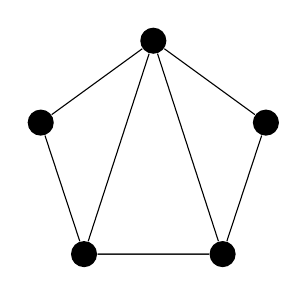
\begin{tikzpicture}
            \node[fill, circle] (V1) at (0,1.5) {};
            \node[fill, circle] (V2) at (1.43,0.46) {};
            \node[fill, circle] (V3) at (0.88,-1.21) {};
            \node[fill, circle] (V4) at (-0.88,-1.21) {};
            \node[fill, circle] (V5) at (-1.43,0.46) {};

            \draw[thin] (V1) -- (V2) -- (V3) -- (V4) -- (V5) -- (V1);
            \draw[thin] (V1) -- (V3)  -- (V4) -- (V1);
        \end{tikzpicture}
        
    Exemplo com $n=5$.
    \end{center}
\end{proof}

\cite{block} ainda mostrou que $b(n)\geq \frac{25}{8}n-o(1)$.

\section {Conjuntos em posição convexa}
Para conjuntos de pontos e posição estritamente convexa, pode-se obter resultados melhores. \cite{blockers} mostrou que, nesse caso, $b(P)=\omega(nlogn)$.

\begin{teorema}[\cite{blockers}]
Se $P$ é um conjunto de $n$ pontos em posição geral e estritamente convexa, então:

    $$b(P)\geq
    \begin{cases}
        n\sum_{k=1}^m\frac{1}{k} \text{ se }n=2m+1\text{ é ímpar}\\
        1+n\sum_{k=1}^{m-1}\frac{1}{k} \text{ se }n=2m\text{ é par}\\
    \end{cases}$$
\end{teorema}
\begin{proof}
    Sejam $p_1, p_2, ..., p_n$ os pontos de $P$ em nomeados em sentido horário. Definimos o comprimento $l(p_i, p_j)$ como a quantidade de arestas de $p_i$ a $p_j$ em $conv(P)$, ou seja, $l(p_i, p_j) = min\{j-i, n+i-j\}$.

    Seja $Q$ um conjunto que bloqueia a vizibilidade de $P$ e $q\in Q$. Percebam que se $q$ bloqueia os segmentos $\overline{p_{i_k}p_{j_k}}$, com $l=min_k{l(p_{i_k},p_{j_k})}$, então $q$ bloqueia no máximo $l$ pares de pontos de $P$.

    Assim, se dermos pesos $\frac{1}{l(p_i,p_j)}$ para cada segmento $\overline{p_ip_j}$, cada $q\in Q$ bloqueia segmentos com soma no máximo $1$. Mas para bloquear todos, precisamos de pelo menos pontos que bloqueiem a soma de todos os pesos.
    Assim:

    $$b(P)\geq |Q|\geq \sum_{i=1}^{n}\sum_{j=i+1}^{n}\frac{1}{l(p_i,p_j)}$$

    Listando os segmentos em outra ordem e sendo $m=\floor{\frac{n}{2}}$, podemos escrever a mesma soma como

    $$\sum_{i=1}^{n}\sum_{j=i+1}^{n}\frac{1}{l(p_i,p_j)} = 
    \begin{cases}
        \sum_{i=1}^n\sum_{j=i+1}^{i+m}\frac{1}{l(p_i, p_j)} \text{ se }n\text{ é ímpar}\\
        \sum_{i=1}^n\sum_{j=i+1}^{i+m-1}\frac{1}{l(p_i, p_j)} + 1 \text{ se }n\text{ é par}\\
    \end{cases}=
    \begin{cases}
        n\sum_{k=1}^m\frac{1}{k} \text{ se }n=2m+1\text{ é ímpar}\\
        1+n\sum_{k=1}^{m-1}\frac{1}{k} \text{ se }n=2m\text{ é par}\\
    \end{cases}$$
\end{proof}

